\documentclass[oneside,a4paper,11pt]{book}


\usepackage{geometry}
 \geometry{
 a4paper,
 total={170mm,257mm},
 left=20mm,
 top=30mm,
 bottom=20mm,
 }


\usepackage{amsfonts}
\usepackage{amssymb}
\usepackage{amsmath}
\usepackage{mathtools}
\usepackage{multicol}
\usepackage[breaklinks=true,hidelinks]{hyperref}
%\usepackage[anythingbreaks]{breakurl}
%\usepackage[hyphens]{url} 
\usepackage{array}
\usepackage{collcell}
\newcolumntype{f}{>{\collectcell\lstinline}l<{\endcollectcell}}
\usepackage{graphicx}
\usepackage{wrapfig}
\usepackage{bm}
\usepackage{xfrac}
%\usepackage{listings}
\usepackage[autolinebreaks,useliterate]{mcode}
\lstset{basicstyle=\lstbasicfont\normalsize}
\usepackage{letltxmacro}
\newcommand*{\SavedLstInline}{}
\LetLtxMacro\SavedLstInline\lstinline
\DeclareRobustCommand*{\lstinline}{%
  \ifmmode
    \let\SavedBGroup\bgroup
    \def\bgroup{%
      \let\bgroup\SavedBGroup
      \hbox\bgroup
    }%
  \fi
  \SavedLstInline
}

\usepackage{float}
\usepackage{fancybox}
\def\figurename{\textsc{Figure}}

\usepackage{caption}
\usepackage{subcaption}

\usepackage{ifthen}
\newboolean{firstanswerofthechapter}

\usepackage{xcolor}
\definecolor{Blue1}{HTML}{1FABD5}
\definecolor{Blue2}{HTML}{1D8DB0}
\definecolor{Blue3}{HTML}{116E8A}
\colorlet{LightBlue}{Blue2!20!white}

\setlength\parindent{0pt}

\usepackage{chngcntr}
\usepackage{stackengine}

\usepackage{tasks}
\newlength{\longestlabel}
\settowidth{\longestlabel}{\bfseries viii.}
\settasks{label={\roman*.}, label-format={\bfseries}, label-width=\longestlabel,
    item-indent=30pt, label-offset=2pt, column-sep={10pt}}
    
%% FONT
%\usepackage{cmbright}
\usepackage{sansmath}
\sansmath
%\DeclareMathVersion{sans}
\SetSymbolFont{operators}   {sans}{OT1}{cmss} {m}{n}
\SetSymbolFont{letters}     {sans}{OML}{cmbrm}{m}{it}
\SetSymbolFont{symbols}     {sans}{OMS}{cmbrs}{m}{n}
\SetSymbolFont{largesymbols}{sans}{OMX}{iwona}{m}{n}
\usepackage[scaled]{helvet}
\renewcommand{\familydefault}{\sfdefault}
\usepackage[T1]{fontenc}
\usepackage[utf8]{inputenc}


%\usepackage{times}


%% EXERCISE STYLE
\usepackage[lastexercise,answerdelayed]{exercise}
\counterwithin{Exercise}{chapter}
\counterwithin{Answer}{chapter}
\renewcounter{Exercise}[chapter]
\newcommand{\QuestionNB}{\bfseries\arabic{Question}.\ }
\renewcommand{\ExerciseHeader}{\noindent\def\stackalignment{l}% code from https://tex.stackexchange.com/a/195118/101651
    \stackunder[0pt]{\colorbox{Blue1}{\textcolor{white}{\textbf{\LARGE\ExerciseHeaderNB\;\large\MakeUppercase{\ExerciseName}}}}}{\textcolor{Blue2}{\rule{\linewidth}{2pt}}}\medskip}
\renewcommand{\AnswerName}{Exercises}
\renewcommand{\AnswerHeader}{\ifthenelse{\boolean{firstanswerofthechapter}}%
    {\bigskip\noindent\textcolor{Blue1}{\textbf{CHAPTER \thechapter}}\newline\newline%
        \noindent\bfseries\emph{\textcolor{Blue1}{\AnswerName\ \ExerciseHeaderNB, page %
                \pageref{\AnswerRef}}}\smallskip}
    {\noindent\bfseries\emph{\textcolor{Blue1}{\AnswerName\ \ExerciseHeaderNB, page \pageref{\AnswerRef}}}\smallskip}}
\setlength{\QuestionIndent}{16pt}
\setlength{\QuestionBefore}{1em}

%% HEADER
\usepackage{svg}
\usepackage{fancyhdr}
\usepackage{titlesec}
\usepackage{tikz}
\usepackage{lipsum}
\usepackage{etoolbox}
\usepackage{enumitem}
\patchcmd{\chapter}{\thispagestyle{plain}}{\thispagestyle{fancy}}{}{}
\usepackage{caption}

\usepackage{pgfplots}
\usepackage{ifthen}

\usetikzlibrary{calc}
\renewcommand{\headrulewidth}{0pt}

\renewcommand{\chaptername}{Assignment}

\pagestyle{fancy}
\fancyhf{}
\fancyhead[C]{%
\begin{tikzpicture}[overlay, remember picture]%
    \fill[Blue2] (current page.north west) rectangle ($(current page.north east)+(0,-1in)$);
    \node[anchor=north west, text=white, font=\Large, minimum size=1in, inner xsep=5mm, align=left] at (current page.north west) {\bf{NONLINEAR SYSTEMS} \\ Assignments};
    \node[anchor=north east, minimum size=1in, inner xsep=5mm] at (current page.north east) {\includesvg[scale=1]{logo.svg}};
      %node[minimum width=\x2-\x1, minimum height=2cm, draw, rectangle, fill=blue!20, anchor=north west, align=left, text width=\x2-\x1] at ($(current page.north west)$) {\Large\bfseries \quad #1};
\end{tikzpicture}
}
\fancyfoot[CO]{
    \begin{tikzpicture}[overlay, remember picture]%
    \fill[Blue2] (current page.south west) rectangle ($(current page.south east)+(0,.5in)$);
    \node[anchor=south west, text=white, font=\large, minimum size=.5in, inner xsep=5mm] at (current page.south west) {\leftmark};
    \node[anchor=south east, text=white, font=\Large, minimum size=.5in] at (current page.south east) {\thepage};
\end{tikzpicture}
}
\fancyfoot[CE]{
    \begin{tikzpicture}[overlay, remember picture]%
    \fill[Blue2] (current page.south west) rectangle ($(current page.south east)+(0,.5in)$);
    \node[anchor=south west, text=white, font=\large, minimum size=.5in, inner xsep=5mm] at (current page.south west) {\leftmark};
    \node[anchor=south east, text=white, font=\Large, minimum size=.5in] at (current page.south east) {\thepage};
\end{tikzpicture}
}
\setlength{\headheight}{12pt}

%% CHAPTER STYLE
\usepackage{titlesec}
\usepackage{tikz}
\usetikzlibrary{calc} 

\titleformat{\chapter}[display]
{}
{\hfill \tikz[remember picture] \node[] (nr) {\bf{\fontsize{20}{70}\selectfont\color{black}ASSIGNMENT~~ \fontsize{60}{70}\selectfont\color{black}\thechapter}};
\begin{tikzpicture}[overlay,remember picture]
\coordinate (rightborder) at ($(nr)+(100,0)$);
\coordinate (right) at ($(nr.east) + (0.5,0)$);
\draw[line width=4.5em, Blue2] (right) -- (rightborder);
\end{tikzpicture}}
{-1ex}
{\filleft\fontsize{30}{50}\selectfont}
[\vspace{-1ex}]

%% TITLE
\author{Prof. Johan Suykens \& Prof. Dirk Roose \\
Teaching assistants: Henri De Plaen \& Thijs Steel}
\title{Nonlinear systems 2020: assignments}
\date{\today}

%%%%% OLD
% ----------------------------------------------------------------
\vfuzz2pt % Don't report over-full v-boxes if over-edge is small
\hfuzz2pt % Don't report over-full h-boxes if over-edge is small
% THEOREMS -------------------------------------------------------
\newtheorem{thm}{Theorem}[section]
\newtheorem{cor}[thm]{Corollary}
\newtheorem{lem}[thm]{Lemma}
\newtheorem{prop}[thm]{Proposition}
\newtheorem{alg}[thm]{Algorithm}
\newtheorem{ex}[thm]{Example}
%\theoremstyle{definition}
\newtheorem{defn}[thm]{Definition}
%\theoremstyle{remark}
\newtheorem{rem}[thm]{Remark}
%\numberwithin{equation}{section}
% MATH -----------------------------------------------------------
\newcommand{\norm}[1]{\left\Vert#1\right\Vert}
\newcommand{\abs}[1]{\left\vert#1\right\vert}
\newcommand{\set}[1]{\left\{#1\right\}}
\newcommand{\Real}{\mathbb R}
\newcommand{\eps}{\varepsilon}
\newcommand{\To}{\longrightarrow}
\newcommand{\BX}{\mathbf{B}(X)}
\newcommand{\A}{\mathcal{A}}
\renewcommand{\d}{\mathrm{d}}
\newcommand{\e}{\mathrm{e}}
\newcommand{\pj}[1]{\textcolor{black}{#1}}
\usepackage{xcolor}
\definecolor{skyblue}{RGB}{48,193,247}
%\newcommand{\rema}[1]{\textcolor{skyblue}{\textit{#1}}}
\newcommand{\rema}[1]{\textcolor{black}{\textit{#1}}}
% ----------------------------------------------------------------
\begin{document}
\vfill
\begin{flushleft}
\vspace*{3cm}
{\textbf{\Huge\color{black}NONLINEAR SYSTEMS}} \\[0.7cm]
{\textbf{\LARGE\color{gray}Assignments}}
\end{flushleft}

\begin{flushright}
\vspace*{1cm}
\textbf{Prof. Johan Suykens \\ Prof. Dirk Roose}\\
\vspace*{1cm}
{\bf\textcolor{gray}{Assistants}}\footnote{Former assistants: Pieterjan Robbe, Joachim Schreurs, Micha\"el Fanuel, Korneel Dumon, Emanuele Frandi, Kris De Brabanter, Ward Melis, Nico Scheerlinck, Marko Seslija.} \\
\textbf{Henri De Plaen \\ Thijs Steel}
\end{flushright}
\vspace*{1cm}

\begin{center}
%\input{attractor.tikz}
\includegraphics[width=0.7\textwidth]{attractor.png}
\end{center}

%\pagenumbering{gobble}

\vspace*{0.5cm}
\begin{center}
    April 2020
\end{center}
\newpage
\vspace*{\fill}
{\Large \bf General guidelines}
\\ \\
This course is evaluated by means of a set of homework assignments (the student is required to make an individual report), which involve the study of a number of dynamical systems via analytical derivations, numerical simulations and bifurcation calculations. In order to help you getting through these assignments, a number of guided sessions are organized. \\ \\
Each session is focused around one exercise, and is meant to get you started. It is impossible to finish the exercise within the session; instead, you should make sure that you know how to proceed independently. Also, at the beginning of each session, we will take a little time to deal with questions regarding the previous exercise. You are therefore encouraged not to leave the assignments until the end of the semester. Note that we cannot (and do not intend to) give all the answers to the assignments during the exercise sessions, since these count as the examination.
\vspace*{\fill} 

\newcounter{session}
\begin{center}
\colorbox{LightBlue}{\parbox{1\textwidth}{\newline
{\noindent 
\begin{list}
{\bfseries\upshape Session \arabic{session}:}
{\usecounter{session}
\setlength{\labelwidth}{2cm}\setlength{\leftmargin}{2.6cm}
\setlength{\labelsep}{0.5cm}\setlength{\rightmargin}{1cm}
\setlength{\parsep}{0.05ex plus0.2ex minus0.1ex}}%\setlength{\itemsep}{0ex plus0.2ex}}
\item Wednesday 26/02 \quad (week 9)
\begin{enumerate}
	\item[a)] \pj{Introduction to software: \lstinline{PPLANE} }
  \item[b)]  Stability of equilibrium points and bifurcations
\end{enumerate}
\item Wednesday 11/03 \quad (week 11)
\begin{enumerate}
	\item[a)] Introduction to software: \lstinline{COCO} \
  \item[b)]  Imperfect bifurcations
\end{enumerate}
\item Wednesday 18/03 \quad (week 12)  \\ \qquad Predator-prey model
\item Wednesday 01/04 \quad (week 14) \\ \qquad Aero-elastic galloping
\item Wednesday 22/04 \quad (week 17)  \\ \qquad Lorenz attractor, Chua and Duffing oscillator
\item Wednesday 06/05 \quad (week 19)  \\ \qquad Pattern formation
\end{list}}}}
\end{center}

\vspace*{\fill}

\newpage


\chapter{Stability of equilibrium points and bifurcations}

\begin{center}
\colorbox{LightBlue}{\parbox{1\textwidth}{\noindent{\bf Note:} There is no need to repeat the information provided during the guided session. Answer the questions as concise and accurate as possible. Use graphical and/or tabular presentation rather than full sentences. The \textit{page limit} 
for this exercise is \textit{4 printed pages}, including figures.}}
\end{center}

% \section{Bead on a tilted wire}

% A bead with mass $m$ moves along a wire, tilted with angle
% $\theta$. A spring with length $L_0$ in relaxed state and with
% spring constant $k$, is fixed to the bead. The motion of the bead
% is damped by a friction force $b\dot{x}$. The construction is
% shown in the following figure.

% \begin{center}
%     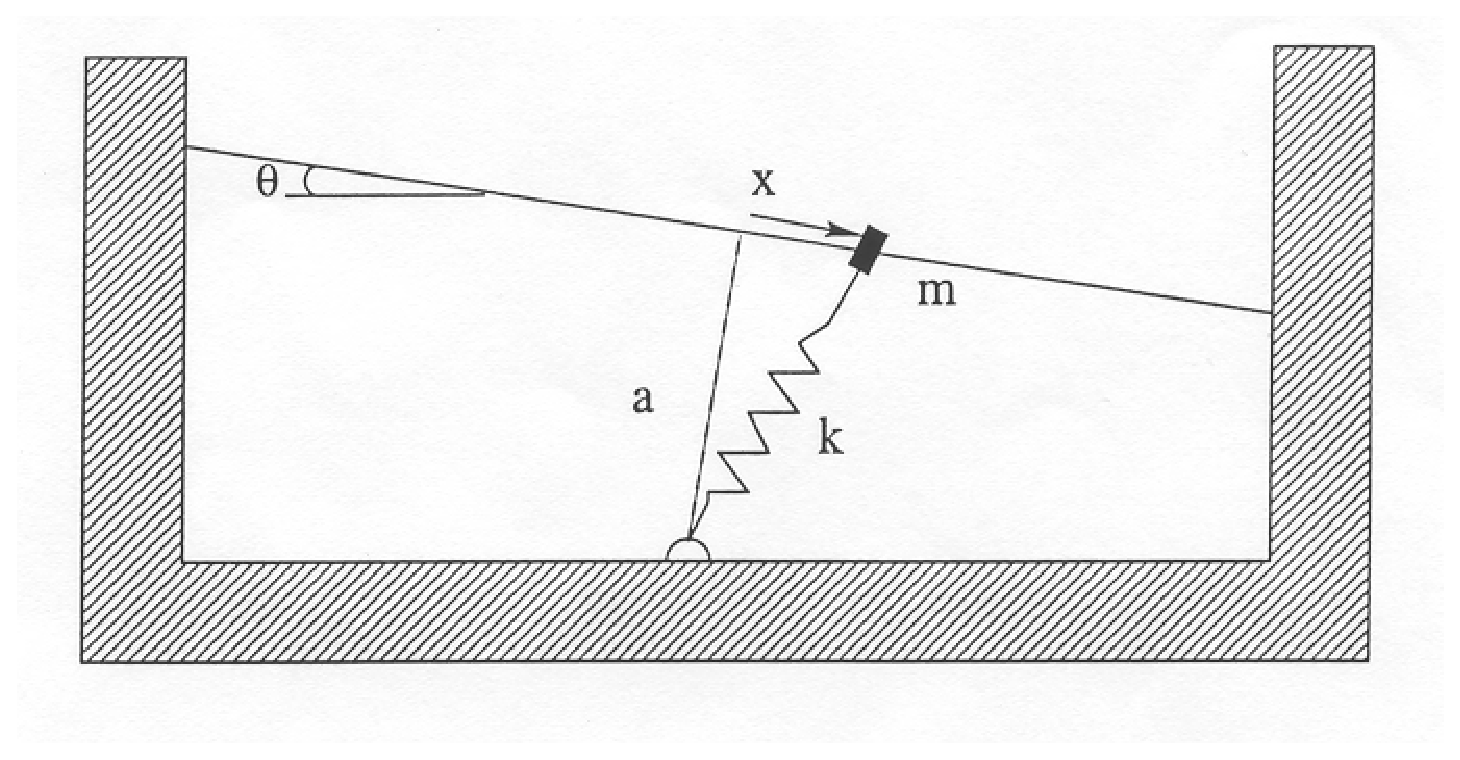
\includegraphics[scale=0.4]{bead}
%     %width=480pt,height=600pt
% \end{center}

% \subsection{System model}

% Given the system model of the bead on a tilted wire
% \begin{equation*}
% m\frac{d^2x}{dt^2}=mg\sin\theta -b\frac{dx}{dt}-kx\left(1-\frac{L_0}{\sqrt{x^2+a^2}}\right).
% \end{equation*}

% \subsection{The case $\theta=0$}

% \begin{enumerate}

% \item Give all fixed points in terms of $k, a, m, b$ and $L_0$.

% \item What is their stability in the case that also $m=0$? Draw a bifurcation diagram for a suitable
% free parameter.

% \item For which relative value of $m$ (different from 0) can the inertia term be neglected and the system be reduced to a first order system? \\
% \textbf{Hint:} make the system dimensionless by dividing by $ak$.

% \item Show that the original differential equation can be transformed to
% \begin{eqnarray*}
% \frac{\partial u}{\partial \tau} & = & v \\
% \frac{\partial v}{\partial \tau} & = & - \frac{1}{\epsilon} [v + (1- \frac{R}{\sqrt{1+u^2}}) u ] \\
% \end{eqnarray*}
% and compare the behaviour via simulation with the behaviour of the
% first order system
% \[ \frac{\partial u}{\partial \tau} = - (1- \frac{R}{\sqrt{1+u^2}}) u \]
% for a fixed $R<1$ (R value depends on your group) and several
% values of $\epsilon$.  To this end, you can use Matlab's
% \verb!ode45! solver.

% \end{enumerate}

% \subsection{The case $\theta \neq 0$}

% \begin{enumerate}

% \item Show that the equilibrium equation can be rewritten in dimensionless form as :
% \[ 1 - \frac{h}{u} = \frac{R}{\sqrt{1+u^2}}\]
% when making an appropriate choice for $R, h$ and $u$.

% \item Give a graphical analysis of the dimensionless equilibrium equation for the cases $R>1$ and $R<1$. How many fixed points can exist in each case?

% \item Show that the equilibrium equation for $r=R-1$ can be reduced to
% \[ - \frac{1}{2}u^3 +ru + h \simeq 0 \]
% when $r, h$ and $u$ are small. Find an approximating formula for the saddle node bifurcation curves in this limiting case.

% \item Show that the exact equations for the saddle node bifurcation curves can be written in following parametric form:
% \[  h(u) = -u^3 \ \ \ \ \ R(u)=(1+u^2)^{\frac{3}{2}}  \]
% when $-\infty < u < \infty$. Give an accurate plot of the bifurcation curves in the $(r,h)$-plane.

% \item Interpret the results physically, in terms of the original variables.

% \end{enumerate}

% https://www.opendatanetwork.com/entity/310M200US16740/Charlotte_Metro_Area_NC_SC/demographics.population.count?year=2016

\begin{Exercise}[name=A simple population model]\label{EX11}


\pj{The population of Belgium could be modeled as
\begin{equation*}
\dot{N} = \alpha \dfrac{(K-N)}{K}N - \beta N,
\end{equation*}
where $N$ is the number of inhabitants, $K$ is the carrying capacity, $\alpha>0$ is the per capita growth rate, and $\beta>0$ is the per capita mortality rate.}

\Question Study the equilibrium points and their stability as a function of $\alpha$ and $\beta$. Summarize your conclusions by using a table. \pj{Which type of bifurcation occurs?} \rema{Answer with a table and/or figures.} 
\Question Based on data from Eurostat\footnote{\url{https://ec.europa.eu/eurostat/web/population-demography-migration-projections/data/database}}, we can estimate a growth rate of $\alpha=1.09\%$ and a mortality rate of $\beta=0.97\%$ in 2016\footnote{$118\,319$ births and $109\,666$ deaths, neglecting emigration, immigration, acquisition or loss of nationality. The total population was 11 311 117.}. Assume the carrying capacity to be $K=15.3$ million. In 2016, the number of inhabitants was $11\,311\,117$. Describe qualitatively what will happen with the population as $t\rightarrow\infty$, according to this model.

%Consider the system for a non-negative real variable $x$ given by:
%
%\begin{equation*}
%\dot{x} = \alpha x (1- \frac{x}{N})-\beta x,
%\end{equation*}
%
%\noindent
%Where $N > 0, \alpha \geq 0$ and $\beta \geq 0$. The growth of $x$ is logistic and the degradation is linear. Study the equilibrium points and their stability as a function of $\alpha$ and $\beta$. Summarize your conclusions by using a table. Identify the type of bifurcation encountered. 
\end{Exercise}

\newpage

\begin{Exercise}[name=Gene control model]\label{EX12}

Consider the coupled system describing the time evolution of non-negative real number numbers $x$ and $y$ given by:
\begin{equation*}
\left\{
    \begin{aligned}
\dot{x} &= \frac{\alpha_1}{1+ y^r} - x, \\
\dot{y} &= \frac{\alpha_2}{1+ x^r} - y,
\end{aligned}
\right.
\end{equation*}


\noindent
where $\alpha_1 \geq 0$, $\alpha_2 \geq 0$ and $r \geq 0$. This model could describe protein abundances of genes. The first term on the right hand side of the equations represents a repression, the second term \pj{represents} a degradation. 

%\begin{enumerate}
    \Question For \pj{a \emph{repression rate}} $r=0$, find a\pj{nd} classify the fixed points. 
    \Question Consider the special case $\alpha_1 = \alpha_2 = 2$ and $r\pj{>0}$.% \in \mathbb{R}^{+} $. 
    \begin{tasks}%[label=(\alph*)]
        \task \label{task121}Find an obvious equilibrium point and verify numerically \pj{(e.g., using \lstinline{PPLANE})} that it is the only one for $0 \leq r \leq 2$.
        \task \label{task122}Study the stability of this equilibrium analytically. \rema{Report your results in a table and/or some figures.}
        \task \label{task123}\pj{At which value of the repression rate $r$ do you expect a bifurcation? Identify its type.} %By studying the stability as $r \in \mathbb{R}^{+} $ varies, explain at which value you expect a bifurcation and identify the type. 
        Do you think this kind of bifurcation is likely based on the properties of the system? Verify numerically for some values of $r$.
        \task Draw numerically all the qualitatively different phase portraits in the region of interest that occur as the parameter $r$ is varied. \pj{Sketch} the bifurcation diagram using the information of \ref{task121}, \ref{task122} and \ref{task123}.
    \end{tasks}
%\end{enumerate}

\end{Exercise}
\chapter{Imperfect bifurcations}

\begin{center}
\colorbox{LightBlue}{\parbox{1\textwidth}{\noindent{\bf Note:} There is no need to repeat the information provided during the guided session. Answer the questions as concise and accurate as possible. Use graphical and/or tabular presentation rather than full sentences. The \textit{page limit} 
for this exercise is \textit{6 printed pages}, including figures.}}
\end{center}

\begin{Exercise}[name=Gene control revisited]\label{EX21}

Consider the gene control model from exercise~\ref{EX12}. 
\Question
Replace your sketch of the bifurcation diagram with an accurate bifurcation diagram, obtained with \texttt{COCO}.

\end{Exercise}

\begin{Exercise}[name=Imperfect bifurcations]\label{EX22}

Consider a simplified equilibrium equation with two parameters $r$ and $h$:
\[ - \frac{1}{\pj{3}}u^3 +ru + h = 0, \] in which $r\in [-1,1]$. \\\\
%
Note that the terms \emph{fold point}, \emph{limit point},
\emph{turning point} and \emph{saddle node bifurcation} are all
synonyms, and are used interchangeably in the literature (and \pj{in} this
assignment).
\Question \pj{Use \texttt{COCO} to plot the bifurcation diagram} as a function of $h$ for different values of $r$.
For which values of $r$ can we observe turning points \pj{with respect to} $h$?
When do we encounter a non-generic turning point?
\Question \pj{Use \texttt{COCO} to plot the bifurcation diagram} as a function of $r$ for different values of $h$ (e.g. $h \in \{-0.1, 0, 0.1\}$).
Identify the turning points.
Show the connection with the disappearance of bifurcation points in 1-parameter problems under perturbation of the model. \pj{What is the meaning of the parameter $h$?}
\Question For the 2-parameter problem, determine the fold curve (i.e., the branch of turning points).
Draw the projection of the fold curve in the $(u,r),
(u,h)$ and $(r,h)$ plane. Compare the latter with your previous
analysis. %How does the fold curve evolve in the $(u,r,h)$-space?

\Question The parameters of the continuation strategy in \texttt{COCO} can influence the computed results significantly. Determine the solution branch\pj{es} for $h \in \{-0.0025, -0.0005\}$, using $r$ as parameter. 
Experiment with the parameters (continuation step length \pj{\texttt{h\_min} and \texttt{h\_max}}, maximum number of %Newton 
iterations \pj{\texttt{ItMX}}, etc.) of the continuation
process \pj{in \texttt{COCO}}. \pj{What is the meaning of these parameters?} When does the numerical procedure lead to wrong results? \rema{Report your findings in a table and/or some figures.}

\textbf{Hint:} In \texttt{COCO}, there are two different parameters that are labeled \texttt{ItMX}. What is the meaning of these parameters? Pay attention to the difference!
\end{Exercise}

\chapter{Study of a predator-prey model}

\begin{center}
\colorbox{LightBlue}{\parbox{1\textwidth}{\noindent{\bf Note:} There is no need to repeat the information provided during the guided session. Answer the questions as concise and accurate as possible. Use graphical and/or tabular presentation rather than full sentences. The \textit{page limit} 
for this exercise is \textit{6 pages text}, \underline{not} including figures.}}
\end{center}

We consider a predator-prey model
\begin{equation*}
\left\{
    \begin{aligned}
        \dot{x} &= x (x - a) (1 - x) - b x y, \\
        \dot{y} &= xy - cy - d,
    \end{aligned}
\right.
\end{equation*}

in which $a, b, c$ and $d$ are physical parameters.

\begin{center}
\colorbox{LightBlue}{\parbox{1\textwidth}{\noindent The values of the para\-meters $a$ and $b$ are fixed and given to you (see \texttt{parameters.pdf} on Toledo). Try always to stay symbolical as long as possible. The numerical values are meant for the plots and the extreme cases where an analytical solution is very hard to find.}}
\end{center}

\noindent Give a brief ecological interpretation to each term and parameter in the equations. You do not have to continue this interpretation later on in the assignment.

\begin{Exercise}[name={A qualitative study without external influence}]\label{EX31}

We consider the parameter $d=0$, and confine ourselves to
parameter values $c \in [0,1.5]$.


\Question First consider the case $y=0$.  Perform a numerical
simulation for a number of initial values $x_0 \in [0,1.5]$ and
describe briefly the qualitative behaviour of the system as a function of time.
\Question For the two-dimensional problem, compute analytically the steady state solutions and determine for each steady state its stability and the topological structure of the
phase diagram in the neighbourhood. For the equilibria in which
$y=0$, give the slow eigendirection of the stable and unstable nodes, and determine analytically the stable and the unstable manifolds for the saddles. \rema{Report your findings in a table and/or some figures.}

\textbf{Hint:} Use the trace and determinant of the Jacobian matrix \pj{or compute its the eigenvalues} to find the topological structure around an equilibrium as a function of the parameter $c$. 

\textbf{Example:}
For the equilibrium $(c,(c - a)(1-c)/b)$, the Jacobian matrix is given by
\begin{equation} 
J=\left[ \begin{array}{cc} 
c(1+a-2c) &  -b c \\
(c-a)(1-c)/b &  0 
\end{array} \right] \nonumber
\end{equation}
The trace $\tau = c(1+a-2c)$ is zero if $c=0$ or $c = (1+a)/2$. The determinant $\Delta = c(c-a)(1-c)$ is zero if $c=0$, $c=a$ or $c=1$. 

\Question Confirm your analysis by drawing phase diagrams for some (relevant) values of $c$. 
Make sure your results are consistent with your analysis in item 2. What is the relation between (stable and unstable) manifolds
of saddle points and separatrices? How can you find the separatrices using a
combination of analytical and numerical techniques?  Determine the
regions of attraction of the attractors. \rema{Answer with some figures.}

\Question Use the results of the previous questions to give a
qualitative overview of the changes in the phase diagram when $c$
varies in $[0, 1.5]$. Give a qualitative picture of the evolution
of the eigenvalues of the Jacobian in the complex plane for the
steady state $(c,(1-c)(c-a)/b)$ as a function of the parameter $c$ and indicate which bifurcations occur.  

\Question Given the interval $[c_1, c_2]$ (see Toledo): between $c_1$ and $c_2$, an important global bifurcation
phenomenon occurs.  Monitor how the periodic solutions change as
the parameter $c$ changes; also look at the period.  Which
bifurcation occurs? At which value of $c$? Can you confirm the bifurcation with a scaling law for the period and/or amplitude of the limit cycles close to the bifurcation?  Draw the phase diagram
for the critical value of $c$.

\Question Compare the evolution of $x$ and $y$ as a function of time
for
\begin{tasks}
\task a limit cycle corresponding to an almost harmonic
oscillation;
\task a limit cycle close to a heteroclinic\footnotemark{} cycle.
\end{tasks}
\rema{Answer with some figures and briefly discuss the qualitative difference between these two
orbits.}

\end{Exercise}\footnotetext{A \emph{heteroclinic} cycle is similar to a \emph{homoclinic} one, at the exception of having multiple centers.}

\begin{Exercise}[name=Bifurcation analysis]

For this part of the assignment, we confine ourselves to $c \in
[0.1, 1.5]$. \textbf{Note:} although this assignment is shorter in text than 3.1, it is equally important (and time-consuming)!

\Question Draw the bifurcation diagram for $d=0$. 
Consider the $(x,c)$ projection.
Discuss the branches, and discuss how the stability changes at all
relevant bifurcation points.  Also compute the periodic solutions.
Make sure that your bifurcation diagram is consistent with the
phase diagrams and analysis of the first part of the assignment.

\Question Draw the bifurcation diagrams for $d=0.01$ and $d=-0.01$; 
Consider both $(x,c)$ and $(y,c)$ projections. 
Compare the results with the bifurcation diagram for $d=0$, and indicate how the transcritical bifurcations disappear. It might be useful to extend your figures to include 
negative values of $x$, $y$ and $c$ to see all branches.

\end{Exercise}

\titleformat{\chapter}[display]
{}
{\hfill \tikz[remember picture] \node[] (nr) {\bf{\fontsize{20}{70}\selectfont\color{black}ASSIGNMENT~~ \fontsize{60}{70}\selectfont\color{black}3b}};
\begin{tikzpicture}[overlay,remember picture]
\coordinate (rightborder) at ($(nr)+(100,0)$);
\coordinate (right) at ($(nr.east) + (0.5,0)$);
\draw[line width=4.5em, Blue2] (right) -- (rightborder);
\end{tikzpicture}}
{-1ex}
{\filleft\fontsize{30}{50}\selectfont}
[\vspace{-1ex}]
    
\chapter{Epidemic Dynamics}
\setcounter{chapter}{3}

\begin{center}
\colorbox{LightBlue}{\parbox{1\textwidth}{\noindent{\bf Note:} There is no need to repeat the information provided during the guided session. Answer the questions as concise and accurate as possible. Use graphical and/or tabular presentation rather than full sentences. The \textit{page limit} 
for this exercise is \textit{2 pages text}, \underline{not} including figures.}}
\end{center}

%%%%%%%%%%%%%%%%%%%%%%%%%%%%%%

\lipsum[1]

\begin{Exercise}[name=Lorem ipsum]

\lipsum[4]

\Question \lipsum[6]

\begin{tasks}

\task First task

\task Second task

\task Third task

\end{tasks}

\Question \lipsum[7]

\Question \lipsum[8]

\end{Exercise}

\begin{Exercise}[name=Dolor sit amet]

\lipsum[10]

\Question \lipsum[11]

\begin{tasks}

\task First task

\task Second task

\task Third task

\end{tasks}

\end{Exercise}

%%%%%%%%%%%%%%%%%%%%%%%%%%%%%%

\titleformat{\chapter}[display]
{}
{\hfill \tikz[remember picture] \node[] (nr) {\bf{\fontsize{20}{70}\selectfont\color{black}ASSIGNMENT~~ \fontsize{60}{70}\selectfont\color{black}\thechapter}};
\begin{tikzpicture}[overlay,remember picture]
\coordinate (rightborder) at ($(nr)+(100,0)$);
\coordinate (right) at ($(nr.east) + (0.5,0)$);
\draw[line width=4.5em, Blue2] (right) -- (rightborder);
\end{tikzpicture}}
{-1ex}
{\filleft\fontsize{30}{50}\selectfont}
[\vspace{-1ex}]
\setcounter{chapter}{3}
\chapter{Aero-elastic galloping}

\begin{center}
\colorbox{LightBlue}{\parbox{1\textwidth}{\noindent{\bf Note:} There is no need to repeat the information provided during the guided session. Answer the questions as concise and accurate as possible. Use graphical and/or tabular presentation rather than full sentences. The \textit{page limit} 
for this exercise is \textit{8 printed pages}, including figures.}}
\end{center}

A constant wind over a flexible, elastic structure can produce or sustain large amplitude oscillations,
as is testified by the Tacoma bridge disaster. One of the mechanisms that can cause this phenomenon is
aero-elastic galloping.\\

\begin{center}
\includegraphics[scale=0.39]{gallop1.jpg}
%width=480pt,height=600pt
\end{center}

\noindent The square prism in the figure above represents an infinitesimal
element of a bridge. The forces that act on the element are:
\begin{itemize}

\item \textit{Inertia} : $m \ddot{y}$

\item \textit{Linear damping}: $r \dot{y}$

\item \textit{Elastic force}: $k y$

\item \textit{Driving force}: The wind speed $V_R$, relative to the prism, is composed of the prism's speed $\dot{y}$ and the constant absolute wind speed $V$. The resulting force depends of the angle $\alpha$ between the relative wind speed $V_R$ and the line perpendicular to the prisms direction of motion. For small $\alpha$, or equivalently large $V$, $\alpha$ can be approximated by $\alpha=\frac{\dot{y}}{V}$. The force along the \textit{direction of the speed} $\dot{y}$ is then given by
\[\frac{1}{2} {\rho V^2 a C(\alpha)}. \]
%(note the difference between $a$ and $\alpha$). We
\pj{We approximate} $C(\alpha)$ by the 7th order polynomial
\[C(\alpha)= A_1 \ \alpha - A_3 \ \alpha^3 + A_5 \ \alpha^5 - A_7 \ \alpha^7, \]
where $\alpha$ is expressed in radials and $A_1=0.04695$,
$A_3=8.932 \times 10^{-4}$, $A_5=1.015 \times 10^{-5}$ and $A_7=2.955 \times 10^{-8}$. Since the
driving force is a function of the speed $\dot{y}$, it can be seen
as a non-linear damping.
\end{itemize}

\noindent In the subsequent analysis, \pj{use} $m=1$, $\rho=1$, $r=1$, $k=100$ and $a=1$.

\begin{enumerate}

\item Write down the equations \pj{for the motion of the prism}. \rema{There is no need to discuss this in your report.}

\item Make a linear approximation of the model. Analyze the stability of \pj{possible} fixed
points as a function of the parameter $V$. At which critical wind speed $V_C$ do we have a bifurcation?
Identify the type of bifurcation of this linear model. Provide a tabular classification of the fixed point. \rema{Answer with a table.}

\item Make a model in \pj{\textsc{Matlab}} of the non-linear model (using the \verb!ode45! solver) where you gradually increase and decrease the parameter $\frac{V}{V_C}$ during the simulation.

\item When looking at the structure of $C(\alpha)$,
use your intuition to describe what will happen in the
neighbourhood of the bifurcation if the non-linear terms are not
neglected\pj{.} Verify using your \pj{\textsc{Matlab}}--model.

\item When $V$ grows larger than $V_C$ another bifurcation happens.
Lowering back $V$ shows the existence of a third bifurcation.
\pj{Identify the type(s) of these bifurcations.}

\textbf{Hint:} plot $y$ as a function of $\dot{y}$.

\item Use \verb!COCO! to obtain
\begin{enumerate}
	\item  a bifurcation diagram, plotting $\frac{A}{V_C}$ as a function of $\frac{V}{V_C}$, where $A$ is the maximal value of $y$ during a period, and
	\item  a plot of the periodic orbits in three dimensions (parameter $\frac{V}{V_C}$ and two phase space coordinates, e.g., $\frac{y}{V_C}$ and $\frac{\dot{y}}{V_C}$).
\end{enumerate}
\pj{Specify the parameters you used to compute the periodic orbits and perform the continuation.} \rema{Answer with some figures.}

\end{enumerate}

\noindent\pj{In the following, make sure that the orbit discretization is not changed between subsequent continuation steps (i.e., set \texttt{NAdapt} equal to \texttt{0}).}

\begin{enumerate}

\item[7.] \pj{The period of a limit cycle can be computed in \texttt{COCO} using}

\pj{\qquad\texttt{period = coco\_bd\_col(po\_data, \textquotesingle po.period\textquotesingle)}.}

\pj{Compute the period of the (first) limit cycle at $\frac{V}{V_C}=1.5$. Experiment with the number of subintervals \texttt{NTST} and the number of collocation points \texttt{NCOL} in each subinterval, while keeping all other parameters fixed. What is the effect on the computed period? Make a tabular representation of the relative error in the computed value for different combinations of \texttt{NTST} and \texttt{NCOL}, e.g., \texttt{NTST} $ \in \{6,12,24,48\}$ and \texttt{NCOL} $ \in \{3,5,7,9\}$. What do you observe?}  \rema{Answer with a table.}

\textbf{Hint:} set \texttt{TOL} to a sufficiently large value for the continuation, but do not change the value for the correction method.


%Implementation details: \\
%see \verb!MATCONT! short reference (by Frank Schilder)
%\begin{itemize}
%	\item  Initialising limit cycle continuation, 
%	\item  Computing branches of limit cycles,  
%	\item  Plotting Results (limit cycles): the function \verb plotcycle \ and computing solution measures. 
%\end{itemize}
%\item Show how the phase portrait evolves
%when varying $V$.  To this end, plot $\frac{\dot{y}}{V_C}$ with
%respect to $\frac{y}{V_C}$ for relevant values of $\frac{V}{V_C}$.

\end{enumerate}

\newpage

\newpage

\chapter{Lyapunov exponents and chaos}

\begin{center}
\colorbox{LightBlue}{\parbox{1\textwidth}{\noindent{\bf Note:} There is no need to repeat the information provided during the guided session. Answer the questions as concise and accurate as possible. Use graphical and/or tabular presentation rather than full sentences. The \textit{page limit} for this exercise is \textit{5 printed pages}, including figures.}}
% I adapted the page limit, because of the abandoned Chau's circuit part. It was 7 previously.
\end{center}


\begin{Exercise}[name=Lyapunov exponents of the Lorenz Equations]
The \textsc{Matlab} source code for this part of the assignment will be distributed during the session. You will get the files \verb$rhs_lorenz.m$ and \verb$lyapunov.m$.  The file \verb$rhs_lorenz.m$ contains the righthand side of the famous Lorenz equations, as well as the corresponding variational
equations.  The file \verb$lyapunov.m$ contains a function that computes and plots the Lyapunov exponents; it takes as input a
function such as \verb$rhs_lorenz.m$ and a number of method parameters.

\Question Take a careful look at this code and explain how/why it computes the Lyapunov coefficients.  What do the variables \verb$st$ and
\verb$kkmax$ mean?  For the Lorenz equations, the Lyapunov exponents are approximately 0.9, 0 and -14.57. Verify this using the \textsc{Matlab} code. Experiment with the method parameters and discuss how they influence the accuracy of the obtained results.
\Question How can you interpret these results? What link can you make between Lyapounov exponents and eigenvalues of fixed points?

\end{Exercise}

\begin{Exercise}[name=The Duffing oscillator]

The Duffing oscillator with periodic forcing can be described by the following differential equation
\begin{equation}
\ddot{x}+k\dot{x}+x^3=B\cos t,
\end{equation}
in which you are asked to choose the model parameters $k$ and $B$ such that the oscillator is in a chaotic regime (see figure). Make sure not to take exactly the same parameter values as a different group. 

\Question Discuss the system behaviour and the sensitivity with respect to the initial conditions.  Illustrate your claims by making use of time plots and phase diagrams.

\Question Repeat this experiment for parameter values in the subharmonic regime and show how this case differs from the chaotic case.

\textbf{Hint: } Transform the Duffing equation to a state space representation. You can then use \textsc{Matlab}'s \verb$ode45$ solver to simulate the time behaviour. See the \textsc{Matlab} help for details.

\Question Use the code from the previous exercise to compute the Lyapunov exponents and discuss.

\vfill
\begin{center}
    \includegraphics[width=0.85\textwidth]{duffing_bis}
    \captionof{figure}{Regimes of the various long-term behaviors of Duffing's equation\footnotemark{},\footnotemark{}}
\end{center}
\vfill

\end{Exercise}\footnotetext[1]{J. M. T. Thompson, H. B. Stewart, \emph{Nonlinear Dynamics and Chaos}, Wiley, 1986.}\footnotetext[2]{Y. Ueda, \emph{Steady motions exhibited by Duffing's equation}, IPPJ--434, 1980.}

% \begin{Exercise}[name=Chua's circuit]

% Consider the following non-linear (but piecewise linear) circuit.

% \noindent The dynamics of this circuit are given by
% \begin{equation*}
% \begin{cases}
% C_1\cfrac{\mathrm{d}v_{C_1}}{\mathrm{d} t} &= G(v_{C_2}-v_{C_1})-g(v_{C_1})\\
% C_2\cfrac{\mathrm{d}v_{C_2}}{\mathrm{d} t} &= G(v_{C_1}-v_{C_2})+i_L\\
% L\cfrac{\mathrm{d} i_L}{\mathrm{d} t} &= -v_{C_2}
% \end{cases}
% \end{equation*}
% with $g(\cdot)$ the piecewise linear characteristic that is depicted in the figure.  The parameter values are chosen to be
% \begin{displaymath}
% \begin{array}{ccccccc}
% \pj{\cfrac{1}{C_1}=11} & \pj{\cfrac{1}{C_2}=2} & \cfrac{1}{L}=7 & G=0.7 &
% m_0=-0.5 & m_1 = -0.8 & B_p = 1
% \end{array}
% \end{displaymath}

% The system can be written as
% \begin{equation*}
% \begin{cases}
% \cfrac{\mathrm{d} x}{\mathrm{d} \tau}&=\alpha(y-h(x))\\
% \cfrac{\mathrm{d} y}{\mathrm{d} \tau}&=x-y+z\\
% \cfrac{\mathrm{d} z}{\mathrm{d} \tau}&=-\beta y
% \end{cases}
% \qquad h(x)=
% \begin{cases}
% bx+a-b &  x > 1\\
% ax & |x|\le 1\\
% bx-a+b & x <- 1
% \end{cases}
% \end{equation*}
% via
% \begin{displaymath}
% \arraycolsep=8pt\def\arraystretch{2.2}
% \begin{array}{lll}
% x=\cfrac{v_{C_1}}{B_p}, & y=\cfrac{v_{C_2}}{B_p}, & z=\cfrac{i_L}{B_pG},
% \\
% \tau=\cfrac{t G}{C_2}, & a=\cfrac{m_1}{G}+1, & b=\cfrac{m_0}{G}+1, \\
% \alpha = \cfrac{C_2}{C_1}, & \beta=\cfrac{C_2}{LG^2}. &
% \end{array}
% \end{displaymath}
% \Question
% Simulate the system behaviour. Show phase portraits in $x,y$ and $z$, as well as individual trajectories starting from two sets of nearby initial conditions.  Illustrate your suspicion about the (chaotic) behaviour of the system.
% \Question
% Use the code from the previous exercise to compute the Lyapunov exponents. %It can be seen that the exponents are clearly wrong. The is caused by the discontinuous function $h$. Try to smooth the piecewise linear model, i.e. the function $h$ and calculate the Lyapunov exponents again using the same code as before.
% \vspace{2cm}
% \begin{center}
% \includegraphics[width=0.55\textwidth]{chua-bis}
% \captionof{figure}{Chua's circuit, a simple autonomous circuit with a chaotic attractor\footnotemark{}.}
% \end{center}

% \end{Exercise}\footnotetext{L. O. Chua, \emph{The Genesis of Chua’s Circuit}, Archiv für Elektronik und Ubertragungstechnik, 46:250-257, 1992.}
\chapter{Pattern formation}

\begin{center}
\colorbox{LightBlue}{\parbox{1\textwidth}{\noindent{\bf Note:} There is no need to repeat the information provided during the guided session. Answer the questions as concise and accurate as possible. The \textit{page limit} for this exercise is \textit{4 printed pages} (\underline{including} figures).}} % I adapted the page limit, because of the abandoned theory part. It was 5 previously.
\end{center}


% \begin{Exercise}[name=Theory]
% Chapter 9 of the book [Misbah]: 
% \Question Prove that the necessary condition for the occurence of a Turing instability 
% is given by (9.9) and that the critical wavevector $q_c$ (which is a scalar for 1D spatial problems) is given by (9.10), starting from (9.2) and (9.3). Show that you understand each step, do not just copy the book.
% \end{Exercise}

\begin{Exercise}[name=Brusselator model]
We consider a system of two interacting species, the famous \emph{Brusselator}
model, which exhibit Turing patterns.  The equations for a one-dimensional spatial domain are given by
%\begin{align*}
\begin{equation}
%\begin{eqnarray}
\begin{array}{ll}
u_t &= D_u u_{xx} + f(u,v) = D_u u_{xx} + A -(B+1)u+u^2v,\\
v_t &= D_v v_{xx} + g(u,v) = D_v v_{xx} + Bu-u^2v,
\end{array}
%\end{eqnarray}
\tag{1}
\end{equation}
%\end{align*}
where $D_u$ and $D_v$ are the diffusion constants of the two species $u$ and
$v$, and $A$ and $B$ are concentrations which are kept constant by coupling
them to a reservoir.  
This is a \emph{activator-inhibitor} model due to the nonlinear coupling term.
The system has a spatially uniform steady state, in which $u_0=A$, $v_0=B/A$.

\noindent
Perform a linear stability analysis of the uniform steady state:
\Question Write the linearization of the Brusselator model around $(u_0,v_0) = (A, B/A)$, cf. section 9.3 of Chapter 9 of [Misbah]
\Question Assume a solution of the form $(u_1, v_1) = (C_u, C_v) e^{iqx} e^{\omega t}$ and write the eigenvalue problem (9.2) for the Brusselator model 
(note that the eigenvector is now denoted as $(C_u, C_v)^T$ instead of $(A, B)^T$ because the symbols $A$ and $B$ are already used to denote concentrations in the Brusselator model. 
\Question Write the dispersion relation (9.4)-(9.5) specifically for the Brusselator model: show that 
\begin{align*}
S &= B - 1 - A^2 -q^2(D_u+D_v),\\
P &= A^2 + q^2(A^2 D_u + (1-B) D_v)+q^4D_uD_v.
\end{align*}
\Question Find the error in formula (9.6). Rewrite the (correct) conditions (9.6) for the Brusselator model.
Check whether conditions (9.12) or (9.13) can be satisfied for the Brusselator model.
%Show that the linear evolution matrix of a Fourier
%mode $(u,v)=(u_1,v_1)\exp(\lambda t + ikx)$ is given by 
%\[\begin{bmatrix}
%(B-1)-D_u k^2 & A^2 \\
%-B & -A^2-D_v k^2
%\end{bmatrix}\]
%\item Calculate the eigenvalues of the linear evolution equation as a function of the wavenumber $k$.
%Show that they are given by the following \emph{dispersion relation},
%\begin{displaymath}
%s_{\pm}=\frac{1}{2}(\Sigma\pm\sqrt{\Sigma^2-4\Delta}),
%\end{displaymath}
%where 
%\begin{align*}
%\Sigma &= B - 1 - A^2 -k^2(D_u+D_v),\\
%\Delta &= A^2 + k^2(A^2 D_u + (1-B) D_v)+k^4D_uD_v.\\
%\end{align*}
%\item When writing $s_{\pm}=\sigma \pm i \omega$, a Turing instability occurs when $\sigma$ changes sign, and $\omega$ is zero.
%Explain this.  
\Question Assume that the diffusion coefficients $D_u$ and $D_v$ and the concentration $A$ are fixed.
For very small values of $B$ the spatially uniform solution is stable.  We would like to increase $B$,
 and are interested in the minimal value for $B$ for which the Turing instability occurs.
Compute $B_c$, the critical value of $B$, and the corresponding critical wavenumber $q_c$.
Show that 
\[q_c=\left(\frac{A^2}{D_uD_v}\right)^{1/4}.\]
and
\[B_c=(1+A\eta)^2,\] 
Here, $\eta=\sqrt{D_u/D_v}$.
\Question When ignoring the diffusion term, one can easily check that the resulting system of two ordinary differential equation
exhibits a Hopf bifurcation when $B=1+A^2$.  \pj{Show that the Turing instability sets in before the Hopf bifurcation when}
\[\eta < \frac{\sqrt{A^2+1}-1}{A}.\]

\end{Exercise}
\begin{Exercise}[name=Numerical experiments]
Use the Matlab-code \verb#brusselator.m# (on Toledo).\\[-.5\baselineskip]

\noindent
The Matlab-code performs time integration of the {\it two-dimensional} Brusselator model, defined on a unit square, i.e.\ Eq.(1) with $u_{xx}$ replaced by $u_{xx} + u_{yy}$ and $v_{xx}$ replaced by $v_{xx} + v_{yy}$. Periodic boundary conditions  and a random initial condition are imposed. Note that in this model the diffusion coefficients are scaled by the actual size of the physical domain, i.e. 
$D_u = \overline{D_u}/L$ and $D_v = \overline{D_v}/L$ where $L$ is the length of each size of the physical square domain and $\overline{D_u}$ and $\overline{D_v}$ are the physical diffusion coefficients.

\Question
Start with the following values: $A=4.5$; $B=7$; $D_u = 1$; $D_v = 8$.
Use the analytical results to check whether the conditions for a Turing instability are satisfied.
Describe what you observe.
\Question 
Lower the value of $B$ so that the conditions for a Turing instability are not satisfied and the homogeneous steady state is stable.  \\
Note that the $u$ (or $v$) values are greycoded so that black and white always correspond to the minimal and maximal values. For a correct interpretation of the values you must check the actual minimal and maximal values (Min and Max).
\Question Reset $B=7$ and increase $L$. Describe what you observe.
\Question Reset the diffusion coefficients and vary $B$ in the interval (6.5,9). Describe what you observe.

\end{Exercise}

% \begin{Exercise*}[name=Reference]
% [Misbah] C, Misbah, \emph{Complex dynamics and morphogenesis}, Springer, 2017.
% \end{Exercise*}


\end{document}
